%\documentclass[12pt,preprint]{aastex}
\documentclass[iop]{emulateapj}
\usepackage{float,amsmath}
%\usepackage[margin=1in]{geometry}
%\usepackage{titlesec} %used to format titles
\usepackage{graphicx} %for handling figures
%\usepackage[none]{hyphenat} %disallows hyphenated words
\newcommand{\vdag}{(v)^\dagger}
\newcommand{\volt}{{v}}
\newcommand{\vis}{{V}}
\newcommand{\sky}{{\rm sky}}
\newcommand{\bmvolt}{{a}}
\newcommand{\beam}{{A}}
\newcommand{\thhat}{{\hat\theta}}
\newcommand{\fngexp}{{e^{\frac{2\pi i\nu\vec{b}\cdot\thhat}{c}}}}
\newcommand{\ifngexp}{{e^{-\frac{2\pi i\nu\vec{b}\cdot\thhat}{c}}}}
\newcommand{\dfngexp}{{e^{2\pi i\nu \Delta \tau}}}
\newcommand{\myemail}{skywalker@galaxy.far.far.away}

%\usepackage{cite}

%\citestyle{aa}
\shorttitle{HERA dish reflectometry }
\shortauthors{Patra et al.}

\begin{document}

\title{THE HYDROGEN EPOCH OF REIONIZATION ARRAY DISH: CHARACTERIZATION OF  THE INSTRUMENTAL RESPONSE WITH REFLECTOMETRY MEASUREMENTS AND ITS IMPLICATIONS ON THE MEASUREMENT OF 21CM POWER SPECTRUM. } 
%\maketitle

\author{Nipanjana Patra\altaffilmark{1} }
\email{Contact author email: nipanjana@berkeley.edu}
\author{Zaki Ali\altaffilmark{1}, Carina Cheng\altaffilmark{1}, Dave DeBoer\altaffilmark{1}}
\author{Gilbert Hsyu\altaffilmark{2}, Tsz Kuk Leung\altaffilmark{2}, Aaron Parsons\altaffilmark{1}}
\altaffiltext{1}{University of California, Berkeley, nipanjana@berkeley.edu}
\altaffiltext{2}{To be inserted}

\begin{abstract}
\end{abstract}


\section{Introduction}

Since it was first proposed in \citep{Shaver_et_al1999} measuring 21~cm
emission from neutral hydrogen in our early universe has gained attention as a
powerful probe of both cosmology and astrophysics.  While the science case for
21~cm cosmology, particularly during the Epoch of Reionization, is well
established (see, e.g.,
\citep{furlanetto_et_al2006,morales_wyithe2010,pritchard_loeb2012}),
the technical path toward measuring this signal has been extremely challenging.  The
weakness of this hyperfine line keeps the 21~cm signal below opacity throughout
cosmological history, but it also creates sensitivity and calibration
challenges that are yet to be fully solved.  With noise temperatures dominated
by sky noise \citep{XXX} and foregrounds four to five orders of magnitude
brighter than the signal \citep{XXX}, 
sky-averaged 21~cm monopole experiments such as
(EDGES; \citealt{XXX}),
(BIGHORNS; \citealt{XXX}),
(SARAS; \citealt{patra_et_al2014}),
(SCIHI; \citealt{voytek_et_al2014}),
(HyPerion; \citealt{presley_et_al2015})
% XXX others?
and 21~cm reionization power spectrum experiments such as
the LOw Frequency ARray (LOFAR; \citealt{XXX}),
the Murchison Widefield Array (MWA; \citealt{XXX}),
the Giant Metre-wave Radio Telescop (GMRT; \citealt{XXX}),
the Donald C. Backer Precision Array to Probe the Epoch of Reionization (PAPER; \citealt{parsons_et_al2010}),
the Hydrogen Epoch of Reionization Array (HERA; \citealt{XXX}),
and the future Square Kilometre Array (SKA; \citealt{XXX})
must
furnish both collecting area and foreground suppression at levels significantly
beyond anything previously achieved in radio telescopes operating below 1 GHz.

One of the most problematic effects facing these experiments is instrument
chromaticity.  The spectral dimension of 21~cm reionization experiments is of vital
importance; for line emission, this coordinate translates to a line-of-sight distance
that can be used to construct three-dimensional maps (and power spectra) of emission,
as well as probe the evolution of 21~cm emission over cosmological timescales.
The evolving response of a radio telescope --- either a single dish
or an interferometer --- versus spectral frequency modulates spectrally smooth foregrounds,
contaminating spectral modes that might
otherwise be used to measure reionization \citep{XXX}.  Moreover, the chromaticity of
a telescope's response scales linearly with diameter, putting the
needs of foreground suppression and signal sensitivity in direct tension with one
another.

A major step forward for the field of 21~cm cosmology has been the development
of a mathematical description of telescope chromaticity, how it varies with
element separation (or telescope diameter), and what it implies for distinguishing
foreground emission from the cosmological 21~cm signal \citep{XXX}.  The ``wedge'', as it is
colloquially known, describes a linear relationship between the separation between elements
in an interferometric baseline and the maximum line-of-sight Fourier mode\footnote{Assuming
a flat sky, and using appropriate
cosmological scalars,
the spectral axis, $\nu$, and angle on the sky, $\vec\theta$, translate to coordinates in
a three-dimensional volume at cosmological distances.  In describing the spatial power spectrum of
emission in this volume $P(\vec k)$, we use the three-dimensional wave vector 
$\vec k\equiv(k_\parallel,\vec k_\perp)$, where $k_\parallel$ is aligned with the
spectral axis $\nu$, and $\vec k_\perp$ lies in the plane of the sky.}
that may be occupied by smooth spectrum foreground emission.  At low-order $k_\parallel$ modes
within the limits of the wedge,
foreground contamination may be suppressed through a combination of calibration and model 
subtraction.  However, calibration or modeling errors rapidly re-establish the characteristic
wedge pattern.  Outside of the wedge, foreground contamination drops rapidly 
\citep{pober_et_al2013,thargarajan_et_al2015}, provided that the spectral responses
of antenna elements and analog electronics are sufficiently smooth\footnote{Here, we distinguish
the chromaticity of the elements in isolation from the chromaticity inherent to
element separation in an interferometric baseline.}.  In promising avoidance-based
foreground strategy employed by PAPER \citep{parsons_et_al2014,ali_et_al2015}, these modes
may be targeted as the lowest risk path for contraining 21~cm reionization in the near term.

In this paper, we examine the performance of a new prototype HERA element in the context of
this new wedge-based framework.  In coordination with \citet{XXXsisterpapers}, we compare 
reflectometry measurements with
a specification for the spectral performance of an element, given models of the relative brightness of
foreground and 21~cm reionization modes in $k$-space.  
% XXX document map



The efficacy of the techniques of foreground removal from the measured data critically limits the 21~cm power spectrum measurements. The delay transformation technique of foreground removal, introduced by  \citep{ParsonsBacker2009,Parsons2012} computes the Fourier transform of the visibility measured by an interferometer and produces a spectrum, referred to as delay spectrum hereafter, which is a function of the geometric time delay corresponding to the physical length of the baseline between two antennas. For the visibilities measured over a wide field across wide frequency bandwidth, the delay spectrum is constituted by the instrument response, the foreground signal and 21cm power spectrum, hereafter referred to as EoR signal.
%The complex visibility measured by an interferometer is a convolution of the instrument response with the true sky response in the UV plane. Therefore, when Fourier transformed, the delay spectrum is the multiplication of the sky response with the instrument response in the delay domain.
The technique exploits the smooth spectral characteristics of the foreground and for a widefield wide bandwidth visibility measurement by an interferometer with a baseline $b$, confines the foreground contribution to the computed delay spectrum within the largest possible time delay $\tau = b/c$ corresponding to the given baseline length. Such techniques also assumes a spectrally smooth instrumental response whose contribution to the measured data, much as the contribution of the smooth spectrum foreground, also has an upper bound in the delay space imposed by the largest geometric delay of the given baseline. 
Beyond this limit, for an ideal system performance, the delay spectrum would be dominated by any wideband signal across the sky with spectral and spatial fluctuation over small scale such as the EoR signal and therefore, could be detectable.\\ 
The interaction between the sky signal and instrument response can alter the relative contribution of the foreground, instrument response and the EoR signal at a given delay and thus influence the detectability of the EoR signal. Such interactions may cause the foreground and systematics to spill over at higher delays and thus push the upper limit of the foreground and systematic contaminated delay modes to much higher delays. In this process, the EoR signal over large spatial scale will be lost.

The Hydrogen Epoch of Reionization Array (HERA) is a proposed array consisting of 568 14-m dishes in South Africa which will measure the 21~cm power spectrum between 100 to 200~MHz.
In this paper, we investigate the performance of the individual HERA elements and resulting contribution of the instrument response to the delay spectrum.
 Reflectometry measurements  are carried out across wide bandwidth on a prototype HERA element in Green
Bank, WV (Figure \ref{fig:heradish}) and the results are interpreted in the light of delay spectrum technique. Section 2 describes the delay spectrum for the ideal and non-ideal performance of a two element interferometer. Reflectometry measurements are described in section 3. Section 4 qualifies the performance of the HERA element as an interferometer for detection of the 21~cm power spectrum.


\begin{figure*}
\centering
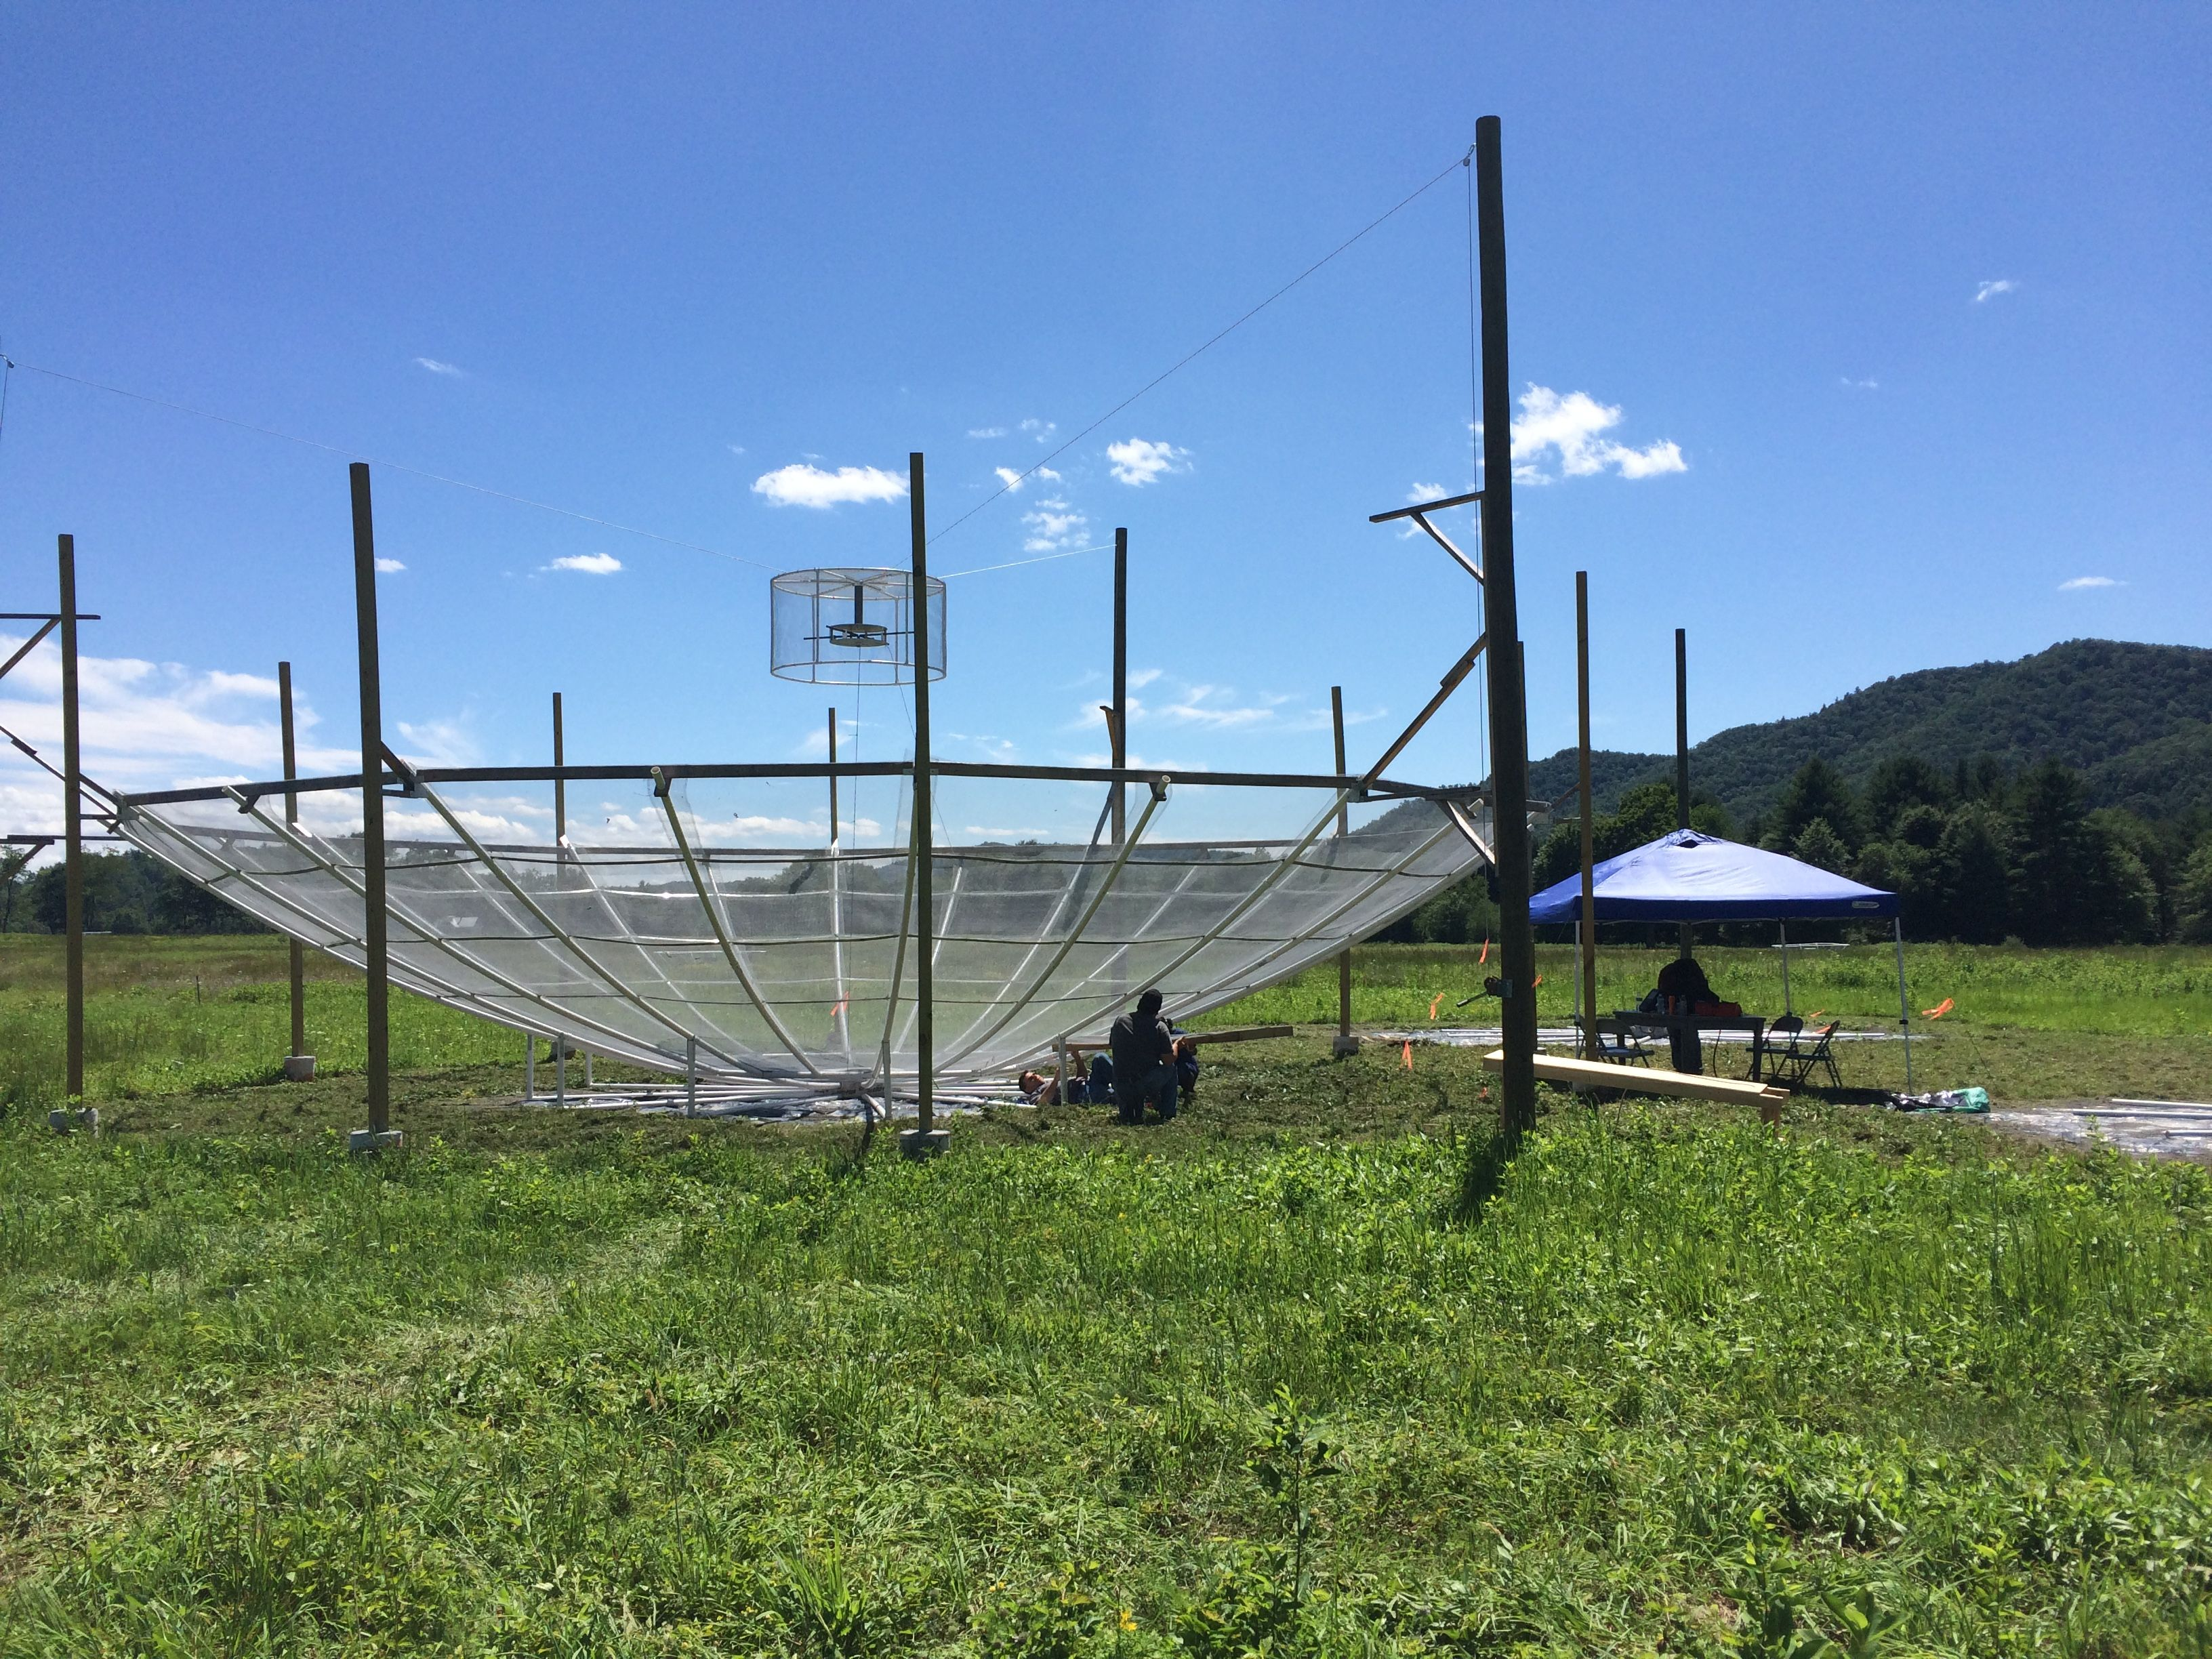
\includegraphics[trim={2cm 20cm 30cm 15cm},clip, totalheight=0.3\textheight]{plots/heradish.jpg}
\caption{HERA dish and feed at the Green Bank NRAO site.}
\label{fig:heradish}
\end{figure*}

\section{Visibility measurements by a two element interferometer and the delay spectrum}

Consider a two element interferometer with a baseline $\vec b$ and antenna field pattern $A(\thhat, \nu)$. If we denote the electric field sky signal in direction $\thhat$ by $\volt_\sky(\vec \theta, \nu)$ and the receiver noise of each element as $\volt_{rec}(\nu)$ then the voltage output of each antenna may be written as,  
\begin{equation}
\volt_{1}(\thhat, \nu) = \bmvolt_{1}(\thhat,\nu)\volt_\sky(\thhat,\nu)\nonumber\\
\end{equation}
\begin{equation}
\volt_{2} (\thhat, \nu)= \bmvolt_{2}(\thhat,\nu)\volt_\sky(\thhat,\nu)\dfngexp\nonumber\\
\end{equation}
where $\bmvolt_{1}(\thhat,\nu)$ and $\bmvolt_{2}(\thhat,\nu)$ are the electric field response patterns 
of the two antennas.
Hence, the time averaged visibility measured by the interferometer may be written as, 
\begin{equation}
\vis(\vec b, \nu) =  \int  \volt_{1}(\thhat,\nu)  \volt_{2}^{*} (\thhat, \nu) \ifngexp d\Omega 
\label{eq1}
\end{equation}

We define antenna cross power pattern as  $\bm(\thhat,\nu)=\bmvolt_{1}(\thhat,\nu)\bmvolt_{2}^{*}(\thhat,\nu)$ and denote the sky intensity as  $I_\sky(\thhat,\nu)=\volt_\sky(\thhat,\nu)\volt_\sky^{*}(\thhat,\nu)$. Hence, 
\begin{equation}
\vis(\vec b,\nu) = \int \bm(\thhat, \nu) I_\sky(\thhat,\nu) \ifngexp d\Omega
	%	& = & \int B(l,m, \nu) I_{sky}(l,m,\nu) exp(-2\pi i \nu \tau_{g} ) dl dm \nonumber\\
 	%	& = & B(\vec u,\nu) \ast P_{sky}(\vec u,\nu ) \nonumber\\
	%	& = & B(\nu { |\vec b| \over c} , \nu) \ast P_{sky}(\nu { |\vec b| \over c} , \nu) \nonumber\\
	%	& = & B(\tau_{g}, \nu) \ast P_{sky}(\tau_{g} , \nu)	
\label{eq2}
\end{equation}

%i.e, the complex visibility is the Fourier transform of the product of the antenna beam pattern with the sky angular power spectrum. In other words, it is the convolution of the Fourier transform of the antenna power pattern with the Fourier transform of the sky. The complex visibility measured by an interferometer with a given baseline length has explicit dependence on frequency as well as implicit frequency dependence through the spatial frequency $\vec u = \nu { \vec b \over c}$ component. Since $\vec u $ is the For a given baseline length $|\vec b|$, the visibility measured at various frequencies are not only the function of frequencies but also samples different $\vec u$ in the uv space. Delay transformation technique takes the visibility measurements at different frequencies and Fourier transforms the complex visibilities. If we defineI_{sky} the Fourier conjugate of the frequency axis as $\tau$ then the equation could be written as, 
In \citet{parsons_et_al2012a}, the Fourier transform of the visibility along the frequency axis was introduced,
resulting in the delay spctrum:
\begin{eqnarray}
\tilde V(\vec b, \tau) & = & \int\!\!\int{\bm(\thhat,\nu) I_\sky(\thhat,\nu) \ifngexp d\Omega~e^{+2\pi i\nu\tau}d\nu}\nonumber\\	                        & = &   \int \left [ A(\thhat, \tau)\ast I_{sky}(\thhat, \tau) \ast \delta( \tau - \frac{{\vec {b} \cdot \thhat}}{c} )\right ] d\Omega 
\label{eq3}
\end{eqnarray}
% XXX rethink how to express this equation (not correct about integrated over all sky)
% XXX define tau_g
The convolution is carried out along the $\tau$ axis which is Fourier conjugate of the frequency $\nu$. In words, the sky delay spectrum from any direction $\thhat$ is convoluted with the delay spectrum of the instrument and would be located at the delay $\tau = {\vec b \cdot \thhat \over c}$ in the delay domain. The maximum geometric delay possible for a given base line would be $\tau_{g} ={ b \over c }$ for the direction of $\thhat = 0$ when the phase centre is halfway in between the two antennas. Hence, the sky contribution from any direction would be confined within $-\tau_{g}<\tau<\tau_{g}$. Due to chromaticity of the sky signal as well as instrument reponse, the delay spectrum of the sky spills over the delay $\tau> \tau_{g}$ with decaying amplitude [Ref to the figure Parsons12]. Sky delay spectrum $I_{sky}(\tau)$ is contributed by the foreground  $I_{fg}(\tau)$  which is spectrally smooth and the 21~cm power spectrum $I_{21}(\tau)$ which contains spectral signatures. Therefore, in the spill over region $(\tau>\tau_{g})$, the relative strength of the smooth spectrum foreground with respect to the delay spectrum of the $I_{21}$ reduces and the 21~cm delay spectrum could potentially be detectable. 

%\subsection{Delay spectrum: An estimate of the 21cm power spectrum}
%Add text here. 
 %\textbf{[ Reference to Nithya's foreground simulation work, reference to any plots on the relative contribution of the  foreground and EoR signal. ]}


\section{Effects of multiple reflections on visibility and delay spectrum}
Response of any radio telescope is chromatic and modulates the true sky signal in the spectral domain. This results in the convolution of the instrument response kernel with the sky signal in the delay domain.
This fundamentally limits the detectability of a 21~cm power spectrum. In this section, the effect of reflections on the visibility data and corresponding effect on the delay spectrum is discussed qualitatively.
 
The Hydrogen Epoch of Reionization Array consists of parabolic dishes which provide increased collecting area per array element compared to its predecessor experiment PAPER. Plane waves incident on a parabolic dish are focussed at the feed which is kept at the focal plane of the dish.
The mismatch between the impedance of free space and the feed and transmission line results in a partial coupling of the sky signal into the feed while the rest is reflected off the feed. 
The reflected signal illuminates the dish and most of it is reflected back into the space.
However, a part of it reflects back and forth several times in between the feed and the vertex of the dish which is shadowed by the feed (dashed blue arrows in Figure \ref{fig:cartoon}).
Such reflections generate multiple copies of the incident sky signal of reduced strength at various delay and phase and thus produces spurious correlations in the visibilities of interferometric data.  Identical spurious visibilities could be resulted due to reflections internal to the system causing delay space distortion. Therefore, it is necessary to measure and understand the instrument delay spectrum in order to qualify the system for the measurement of 21cm power spectrum. 
In this section we compute the visibility of a two element interferometer accounting for the additional reflections of the sky signal in between the feed and the dish vertex and the corresponding effects on the delay spectrum. 

\begin{figure}[ht!]
\centering
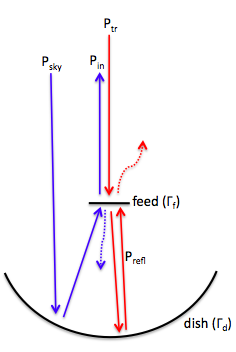
\includegraphics[totalheight=0.35\textheight]{plots/reflection_cartoon.png}
\caption{The propagation path of the sky signal entering the
feed in receiving mode is shown in blue. Due to impedance mismatch between feed and the free space, a part of the signal (dashed blue) is reflected off the feed. This signal reflects off the dish apex several times and returns to the feed at multiple delays with reduced signal strength. The red line shows the signal path during measurements which is done in transmission mode. Appropriate corrections are made to derive the telescope response function during sky observation. }
\label{fig:cartoon}
\end{figure}

Consider again a two element interferometer as described in section 2. Two antennas are assumed to be exactly identical so that their electrical parameters and the field pattern are identical i.e, $a_{1}(\thhat,\nu) = a_{2}(\thhat,\nu)$. We denote the voltage reflection coefficient of each feed by $\Gamma_{f}$. The voltage reflection coefficient of the reflector dish is denoted by $\Gamma_{d}$. Upon first incidence of the sky signal onto the dish, it is reflected from the entire dish and is focussed onto the feed. Hence, for first incidence $\Gamma_{d}=1$. Sky signal that would return to the dish after successive reflections off the feed and the dish is reflected only from a small area around the vertex of the dish and therefore, $\Gamma_{d}<1$. In our analysis, we consider one reflection of the sky power from the feed and subsequent reflection off the dish as one single reflection. If the focal length of the dish is $l$, assuming the feed is located at the focus, the roundtrip delay after first reflection will be $\Delta \tau = {2l \over c}$. 


\subsection{Visibility and delay spectrum computation considering multiple reflections}
Upon first incidence of the sky signal $\volt_{sky}$, $\Gamma_{f}$ fraction of the voltage is reflected off the feed while $(1-\Gamma_{f})$ fraction is coupled to the feed. The reflected voltage then further reflected off the dish and $(1-\Gamma_{f}) $ fraction of it reenters the feed with a roundtrip time delay $\Delta \tau$. Hence, if $I_{sky}$ is reflected n times in between the feed and the dish, the net voltage entering the feed after an
$n^{th}$ reflection off the feed and the dish is written as:
\begin{eqnarray}
\volt_{1} & = &  a_{f} \volt_{sky}[1+ (1-\Gamma_{f})\Gamma_{f}\Gamma_{d} \dfngexp \nonumber \\
	&& + (1-\Gamma_{f})^{2} (\Gamma_{f}\Gamma_{d})^2  (\dfngexp)^{2}+ \nonumber \\
&&  ....+ (1-\Gamma_{f})^{n}(\Gamma_{f}\Gamma_{d})^{n} (\dfngexp)^{n}] \nonumber
\end{eqnarray}
and, 

\begin{eqnarray}
\volt_{2} & = &  a_{f} \volt_{sky}[1+ (1-\Gamma_{f})\Gamma_{f}\Gamma_{d} \dfngexp \nonumber\\
&&+ (1-\Gamma_{f})^{2} (\Gamma_{f}\Gamma_{d})^2  (\dfngexp)^{2}+ \nonumber \\
&& ....+ (1-\Gamma_{f})^{n}(\Gamma_{f}\Gamma_{d})^{n} (\dfngexp)^{n}] \ast \fngexp \nonumber
\end{eqnarray}




%\begin{eqnarray}
%\volt_{1} & = & a \volt_{sky}(1-\Gamma_{f}) + a \volt_{sky} \Gamma_{f} \Gamma_{d} \dfngexp  (1-\Gamma_{f})^{2}\nonumber\\
   %      & = & a \volt_{sky} (1-\Gamma_{f}) \left [ 1+ (1-\Gamma_{a})\Gamma_{f} \Gamma_{d} e^{2\pi i\nu \Delta \tau} \right]\nonumber
%\end{eqnarray}
%\begin{eqnarray}
%\volt_{2} & = & \left [ a \volt_{sky}(1-\Gamma_{f}) + a \volt_{sky} \Gamma_{f} \Gamma_{d} \dfngexp (1-\Gamma_{f})^{2}\right ] \fngexp \nonumber\\
   %      & = & a \volt_{sky} (1-\Gamma_{f}) \left [ 1+(1-\Gamma_{a}) \Gamma_{f} \Gamma_{d} \dfngexp  \right] \fngexp \nonumber
%\end{eqnarray}
Frequency as well as angular dependence of the quantities are not written explicitly for notational simplicity. We also absorb the common gain term $(1-\Gamma_{f})$ with antenna field pattern $a$ and denote them as $a_{f}= a(1-\Gamma_{f})$ here after and define the antenna cross power pattern as $\beam_{f}(\thhat,\nu)=\bmvolt_{f}(\thhat,\nu)\bmvolt_{f}^{*}(\thhat,\nu)$ . 

%\begin{eqnarray}
%\vis(\vec b, \nu) & = & \int \volt_{1}\volt_{2}^{*} d\Omega \nonumber\\
%		        & = & \int \beam_{f} \volt_{sky}|^{2} |\left [ 1+(1-\Gamma_{f}) \Gamma_{f} \Gamma_{d} \dfngexp  \right]|^{2} \fngexp  d\Omega
%\label{eq4}		        
%\end{eqnarray}


 Furthermore, combining all the terms that contain instrument response we define a common instrument parameter, written as, 
 
 
 \begin{eqnarray}
\Sigma(\vec b, \nu) & = & a_{f}  [ 1+ 2 \Re [(1-\Gamma_{f}) \Gamma_{f}\Gamma_{d} \dfngexp \nonumber\\
&& + (1-\Gamma_{f})^{2}(\Gamma_{f}\Gamma_{d})^2(\dfngexp)^{2}+ \nonumber\\
&&  ....+(1-\Gamma_{f})^{n} (\Gamma_{f}\Gamma_{d})^{n}(\dfngexp)^{n} ] ]\\
& = & { a_{f}\over \Gamma_{f} } \displaystyle\sum\limits_{n=1}^{n} [\Gamma_{f}\Gamma_{d}e^{i\phi}]^{n}
   \nonumber\\
   \label{eq6}
\end{eqnarray}
 
 
 
%\begin{eqnarray}
%\Sigma(\vec b, \nu) & = & \bm_{f} |\left [ 1+ (1-\Gamma_{f}) \Gamma_{f} \Gamma_{d} e^{2\pi i\nu \Delta \tau} \right]|^{2}\nonumber\\
 %	    & = &  \bm_{f}  \left[ 1+ |(1-\Gamma_{f})|^{2}|\Gamma_{f}|^{2}|\Gamma_{d}|^{2} + 2 \Re \left ( (1-\Gamma_{f})\Gamma_{f}\Gamma_{d} \dfngexp \right) \right] 
%\label{eq{5}}	    
%\end{eqnarray} 

Instrumental response function acquires additional terms arising due to correlation between the direct and reflected component of the sky signal. Fourier transform of this visibility spectrum along the frequency axis results in the delay spectrum. 
Fourier transform of the visibility contributed by any two voltage components from two antennas with no mutual delay will be located at the same delay $\tau = 0$ in the Fourier domain whereas any two voltage components from two antennas components having a mutual delay of $\Delta \tau$ will be centred at $\tau+\Delta \tau$. This additional delay extends the upper limit on the maximum geometric delay $\tau_{g}$ to $(\tau_{g}+\Delta \tau)$.
 Thus, the correlation between the reflected signal  from the feed and subsequently from the dish with the direct signal extends the foreground response to delays beyond the maximum geometric delay for a given baseline and contaminates the delay mode where 21~cm delay spectrum could potentially be detected. 
 
 %If the dish vertex is so constructed such that the reflection from the dish vertex is negligible i.e, $\Gamma_{d}<<1\ or = 0$ then the second and the third term of the $\Sigma$ vanish. Also, the second term in the expression of $\Sigma(\vec b, \nu)$ is negligible compared to the first and the third term of the expression and, therefore, can be neglected. \\
%===================================

The respective visibility as well as the dealy spectrum would be, 
\begin{equation}\label{eqn:series1}
\vis(\vec b, \nu)  = \int I_{sky}(\vec b, \nu)\Sigma(\vec b, \nu) \fngexp d\Omega
\end{equation}
\begin{eqnarray}
%\tilde V(\vec b, \tau) & = & \int \left [ \int I_{sky}(\vec b, \nu)\Sigma(\vec b, \nu) \fngexp  d\Omega \right ]  e^{-2\pi i\nu\tau} d\nu \nonumber \\
\tilde V(\vec b, \tau) & = & \int \left [ I_{sky}(\thhat, \nu) \ast \Sigma(\thhat, \nu) \ast \delta( \tau - \frac{{\vec {b} \cdot \thhat}}{c} )  \right] d\Omega
\label{eq7}
\end{eqnarray}


The design specification of HERA elements requires that any
signal, arriving at the feed at a delay $\Delta \tau$ with respect to the direct incidence, should be
at the level of $-60dB$ at a delay of $60ns$ relative to the first incident
signal at the feed \citep{parsons_deboer_memo}. This specification was
approximated based on the power level of the cosmological signal in relation to
foreground signals, which is estimated to be six orders of magnitude fainter
\citep{santos_et_al2005,ali_et_al2008,deoliveira2008,jelic_et_al2008,bernardi_et_al2009,bernardi_et_al2010,ghosh_et_al2011}. Additionally, the $14m$ HERA baselines set a foreground containing
horizon-limit (the wedge) that, with some buffer, sets a delay specification of
$60ns$
\citep{parsons_et_al2012b,vedantham_et_al2012,nithya_et_al2013,liu_et_al2014a,liu_et_al2014b}. Our goal is to measure the instrument response $\Sigma(\nu)$ and its effect on the power spectrum measurements. 
%%%%%%%%%%%%%%%
\section{Measurements}
We carried out reflectometry measurements at the HERA element prototype in Green
Bank, WV (Figure \ref{fig:heradish}) in order to measure the instrument response of the feed and dish assembly and characterise its performance. An HERA element consists off a $14\,m$ diameter
parabolic reflector and a crossed-dipole pair as a feed. The cross dipole antenna pair is identical to the feed of the PAPER antenna which is suspended at the focal plane of the dish with the support of three vertical poles. HERA elements are closely spaced with centre to centre distance between two dishes are equal to the dish diameter. Therefore, to reduce the coupling between the adjacent dishes, the crossed dipole feed along with the back plane is encased in a cylindrical cage. The feed is raised and
lowered by a three-pulley system mounted on the three poles. The focal height of the dish is $4.5m$
($\sim{14.76}$ft).  



%As HERA progresses as an experiment, it is necessary to build optimised dishes that aim to minimise the
%challenges of chromaticity in our quest for the Epoch of Reionization.

As given in the previous section, if the incident power from the sky signal is $I_{sky}$, the feed
reflection coefficient is $\Gamma_{f}$, and the dish reflection
coefficient is $\Gamma_{d}$, then the net power entering a feed after
$n^{th}$ reflection off the feed and the dish is:

\begin{eqnarray}
\tilde I_{meas}(\vec b, \nu) & = & \int I_{sky}(\vec b, \nu)\Sigma(\vec b, \nu) \fngexp d\Omega
\end{eqnarray}



where, $\Delta \tau$ is the roundtrip propagation delay of a frequency $\nu$ due to a reflection over the focal distance $l$. $I_{meas}$ is the auto correlated power obtained from a single HERA element. Upon our assumption that two adjacent antenna elements have identical electrical properties, this power is also a measure of the cross power or the visibility $\vis (\vec b, \nu)$ between the two antennas with a normalisation factor of $2$. Once again, it is to be noted that upon the first incidence, the sky signal is focussed onto the feed from the entire dish and the dish reflection coefficient $\Gamma_{d}$ is $1$ for this first incidence. The subsequent back and forth reflection of the signal in between the feed and the dish, however, occurs from only the part of the dish which is shadowed by the feed. Therefore, in this case, $\Gamma_{d} < 1$. For a given baseline $\vec b$, taking the ratio of the measured power and the incident power, 

\begin{eqnarray}\label{eqn:ratio1}
{I_{meas} \over I_{sky} } & = & \Sigma(\vec b, \nu) \nonumber\\
  & = & { a_{f}\over \Gamma_{f} } \displaystyle\sum\limits_{n=1}^{n} [\Gamma_{f}\Gamma_{d}e^{i\phi}]^{n}
   \nonumber\\
   \label{eq8}
\end{eqnarray}

The right hand side of this equation is the instrument response kernel of a single HERA element as well as a representative of the instrument response in the measured visibility data between a pair of antennas. Our goal is to measure this kernel as a function of frequency and determine its effect on the delay spectrum of the visibility. 

%%%%%%%%%%%%%%%%%
\subsection{Method}
The instrument response kernel is measured by measuring the return loss of the antenna element at the output port of the feed using a vector network analyser. The vector network analyser transmits a broadband noise of known amplitude and phase via a $75ft$ cable up to the feed. While a part of this signal  is returns to the VNA post reflection from the feed due to mismatch between the cable and the antenna impedance resulting in the primary return loss, rest of the signal is radiated out by the antenna and illuminates the dish and radiated into the space. However, the reflected signal from the dish vertex returns to
the feed. This incident signal is now
reflected back and forth in between the feed and the dish much like the sky
signal reflection discussed previously.

If $I_{tr}$ is the signal transmitted by the VNA , $\Gamma_{f}$ is the feed reflection coefficient, $I_{r}$
is the power incident back on the feed after reflection from the dish then the reflected power, $I_{refl}$,
back into the VNA would be:
\begin{equation}\label{eqn:series2}
I_{refl} =  I_{r}A_{f}[1+ \Gamma_{f}\Gamma_{d} e^{i\phi}+ (\Gamma_{f}\Gamma_{d})^2e^{i2\phi}+ ....+ (\Gamma_{f}\Gamma_{d})^{n}e^{in\phi}]
\end{equation}
 
Once again, we consider one reflection from the feed and its subsequent reflection from the dish as one reflection in total. Equation \ref{eqn:series2} is similar to Equation \ref{eqn:series1}, with different incident powers.

$I_{r}$ is the power that is incident back on the feed, which is just the feed radiated power reflected off the dish:
 
\begin{equation}
I_{r}= \Gamma_{d}(1-\Gamma_f)e^{i\phi} I_{tr}
\end{equation}

Hence the total returned power $P_{ret}$, to the VNA  would be:

\begin{eqnarray}
I_{ret} & = & \Gamma_{f}I_{tr} \nonumber\\ 
 & + &   \Gamma_{d}(1-\Gamma_f)e^{i\phi} I_{tr}(1-\Gamma_{f}) [1+ \Gamma_{f}\Gamma_{d} e^{i\phi}+  ....+ (\Gamma_{f}\Gamma_{d})^{n}e^{in\phi}]\nonumber\\
 \end{eqnarray}
 
Simplifying:
 
  \begin{eqnarray}\label{eqn:ratio2}
 {I_{ret} \over I_{tr} } & = & \Gamma_{f}
  +  \Gamma_{d}(1-\Gamma_f)^{2} [e^{i\phi}+ \Gamma_{f}\Gamma_{d} e^{i2\phi}+  ....+ (\Gamma_{f}\Gamma_{d})^{n}e^{i n\phi}]\nonumber\\
  & = & \Gamma_{f} + { (1-\Gamma_f)a_{f}\over \Gamma_{f} } \displaystyle\sum\limits_{n=1}^{n} [\Gamma_{f}\Gamma_{d}e^{i\phi}]^{n}
 \label{eq9}
\end{eqnarray}

The ratio in Equation \ref{eqn:ratio2} is the returned power to the VNA with
respect to the transmitted power sent by the VNA. It is identical to the sky
observation case in Equation \ref{eqn:ratio1} but differs by two factors. The
first factor corresponds to an additive amplitude difference arising from
$\Gamma_{f}$, which physically accounts for the initial reflection at the feed.
The second difference is a multiplicative term which informs us about the first
reflection. Both of these terms need to be corrected for in order to relate our
measurements to real observations.
%Therefore, because our measurement is carried out in transmitting mode
%while a sky observation would be carried out in receiving mode, we correct our
%results in order to map them real observations.

The VNA measures the magnitude and phase of the quantity ${I_{ret}\over I_{tr}}$
as a function of frequency as shown in Figure \ref{fig:freq}. The magnitude and phase of the complex return loss is measured between 50 to 500MHz over 1024 frequency channels which gives a frequency resolution of 0.44MHz. The delay resolution of the measurements is ?t = 2.22ns. In our measurement
set-up, the first reflection occurs at the feed $\Gamma_{f}$, so
$({I_{ret} \over I_{tr} }  - \Gamma_{f}) $ gives an estimate of the delay
spectrum of the sky signal. In delay domain, the relative signal strength at
zero delay represents the factor $\Gamma_{f}$ while the signal strength at any
other delay represents any delayed signal that enters the feed after being
reflected from the feed surroundings. 

%\section{Methodology}{\label{sec:methods}}

%Our reflectometry measurements are made using a prototype HERA dish at NRAO in Green Bank, WV. The dish is a $14\,m$ diameter
%parabolic reflector structurally supported with 3 telephone poles. The
%reflective material is made up of wire mesh that is attached to PVC
%pipes, forming the parabolic shape of the dish. With the current iteration of
%the HERA dish, the feed consists of a PAPER dipole encased in a cylindrical cage
%encompassing the backplane. The PAPER feed and the backplane (which is aimed at
%preventing feed-to-feed interaction between neighboring dishes) is raised and
%lowered by a three-pulley system. The focal height of the dish is $4.5m$
%($\sim{14.76}$ft).  

%The heights measured in our experiment were made from
%the balun to the top of the concrete hub. However, the focal height should be
%measured from the backplane to point where the wire mesh would intersect the
%concrete hub at the vertex of the dish. To account for this height discrepency,
%we add 1.96 ft to all of our measured heights. These are the heights quoted in
%the plots.[XXX not done yet but will be done]
%Our measurements are made with a FieldFox in VNA mode. In this mode, a pulse
%is generated in the FieldFox and sent through a $75ft$ $50\Omega$ cable that
%connects to the feed with a 4:1 passive balun. The magnitude and phase of the complex return loss is measured between 50 to $500MHz$ over 1024 frequency channels which gives a frequency resolution of 0.44MHz. The delay resolution of the measurements is $\Delta{t}=2.22ns$.
%In addition, we note that the round trip of a reflection from the feed to the dish
%is $9m$, which corresponds to a delay of $30ns$.


%Feed heights quoted in our measurements represent the distance from the balun to
%the top of the central concrete hub. However, the actual focal height
%of the dish represents the distance from the backplane of the feed to the dish's
%wire mesh, which intersects the concrete hub between the ground and the top of
%the hub. A 
%XXX get discrepancy distance from DaveD. (1.7 ft from the bottom plate of
%sandwich to the top of the the cage and .26 ft from the top of the concrete hub
%to the middle where the parabola starts)

%need to add in third : Antenna feed focal length 4.5 m which corresponds to a
%signal propagation delay of 0.3 ns. Hence, subsequent reflections from the dish
%vertex are expected to be at a delay which is integral multiple of 0.3 nS.
\begin{figure*}
\centering
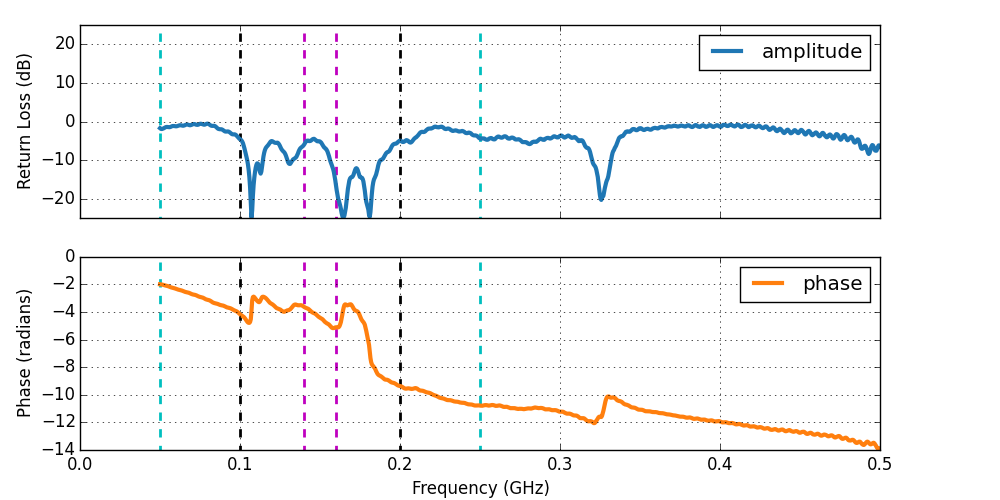
\includegraphics[totalheight=0.3\textheight]{plots/frequency_amp_phase_fullbw.png}
\caption{Amplitude and phase of the measured return loss. Colored dashed lines
mark three different frequency bands: $140-160MHz$ (typical power spectrum bandwidth),
$100-200MHz$ (PAPER bandwidth), and
$50-250MHz$ (HERA bandwidth).}
\label{fig:freq}
\end{figure*}
%++++++++++++++++++++++++++++++++++++++++++++++++++++++

\subsection{Estimation of the delay spectrum of the instrument}
Frequency domain data, as shown in Figure \ref{fig:window}, is Fourier-transformed to compute the response of the system in the delay domain. The signal transmitted by the VNA is reflected first from the feed. In delay domain,  this appears at the zero delay bin. We subtract this value from the measured data and divide the the data by a factor $(1-\Gamma_{a})$ to derive the delay spectrum for the system operating in receiving mode during sky observation.   %Because the measured data is band-limited between $50$ to $500MHz$, it is analogous to multiply the measured data by a square window function. 
%Then in delay domain, the response would be convolved with a $sinc$ function. This may result in excess power at high
%delays due to the sidelobes of the $sinc$ function. Hence, appropriate windowing of the measured data set is necessary before taking the Fourier transform.
%We have chosen a Hamming window for our analysis, and its effectiveness of this
%window function compared to others is illustrated in Figure
%\ref{fig:window}. 

As mentioned in Section \ref{sec:theory}, there is a mismatch in amplitude
between the reflections that we measure (originating from the FieldFox pulse)
and reflections produced by sky signal. The reflections that we measure (at high
delays) must be lowered by a factor to represent weaker reflections that would
occur after most of the sky signal is received by the feed. For our
compensation, we multiply our entire delay spectrum by its DC component, which is the feed reflection coefficient $\Gamma_{f}$, and also divide by ($1-\Gamma_{f}$). In other words, these correction factors equate Equation \ref{eqn:ratio2} with Equation \ref{eqn:ratio1}. 
We note that this correction is only accurate at high delays where our
reflections of interest occur. At low delays, our spectrum amplitude should be
increased to represent the original sky signal, but we do not apply this
correction because it is not relevant to our analysis.

\begin{figure*}
\begin{minipage}[b]{0.5\linewidth}
\centering
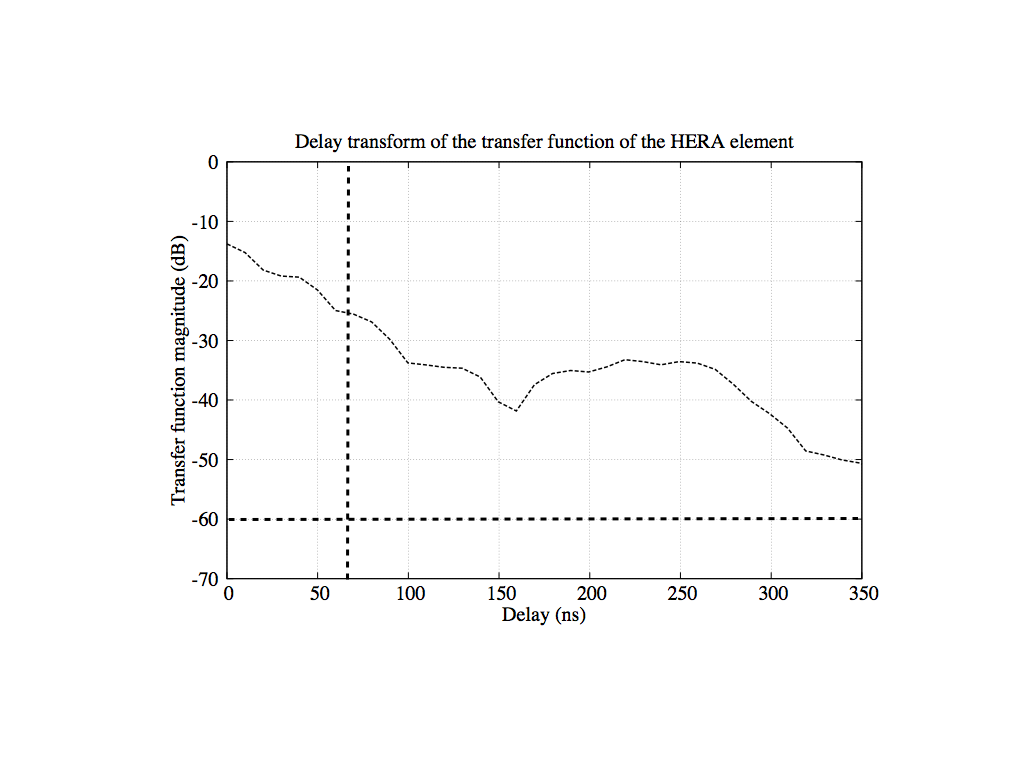
\includegraphics[width=\linewidth]{plots1/delayspectrum.png}
\caption{Delay transform of the transfer function of the HERA element. The complex return loss of the element is measured between 50 to 400~MHz when the feed is kept at the focal plane of the dish at a focal height 4.5m. The delay spectrum is produced by taking the Fourier transform of the magnitude of the return loss measurement after limiting the measurements between 100 to 200~MHzusing Blackman-Harris window. The intersection of the horizontal and vertical dashed line shows the instrument performance specification as predicted by the theory of delay transform in order to detect the 21cm power spectrum.}
\label{fig:window}
\end{minipage}
\begin{minipage}[b]{0.5\linewidth}
\centering
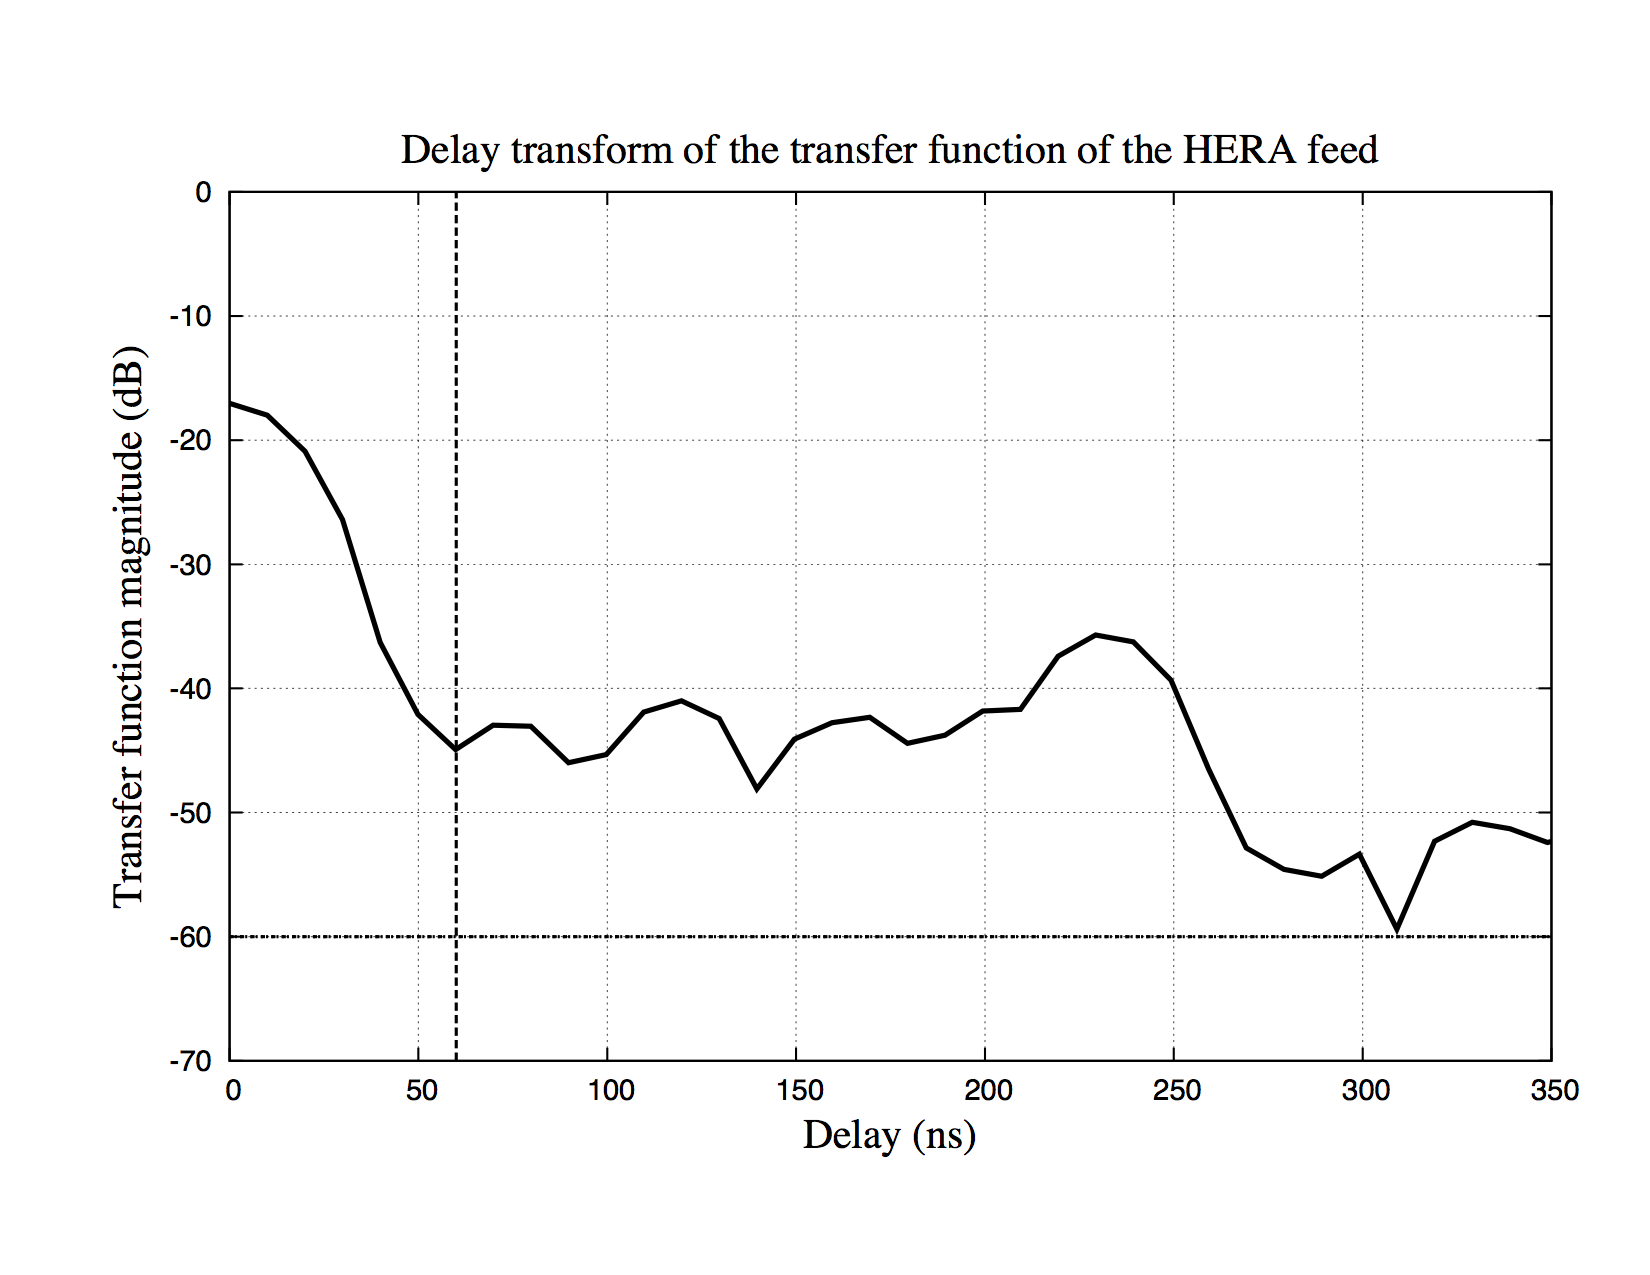
\includegraphics[width=\linewidth]{plots1/delayspectrum_feed.png}
\caption{Delay transform of the transfer function of the HERA feed element. The feed is kept on the ground downside up so that the entire radiation from the feed is radiated out. Once again, the measurement is done between 50 to 450 MHz and the delay spectrum is produced between $100-200$~MHz by using a Blackman-Harris window. The black dashed lines illustrate the instrument specification.}
\label{fig:outofthedish}
\end{minipage}
\end{figure*}

\section{Results}

Figure \ref{fig:freq} shows the return loss for a frequency bandwidth of $50$ to
$500MHz$, measured when the feed is suspended at the focal plane of the parabolic dish which is at $4.26m$ from the dish vertex. 
This measurement is Fourier transformed to obtain the delay spectrum of the instrument in the receiving mode as given in equation \ref{eq3}.
%In Figure \ref{fig:3bands}, the return loss we measure is plotted versus delay
%for three chosen bandwidths: the HERA bandwidth, the PAPER bandwidth, and a
%typical power spectra bandwidth when using a Hamming window function. Two
%additional measurements, using data taken in 2014 with the first prototype HERA
%dish near Berkeley, CA, are also plotted using two different bandwidths. One of
%the main differences between the Green Bank and Berkeley measurements is that
%the feed was not encompassed in a cage for the Berkeley data (only a backplane). Additionally, the $50-1000MHz$ data taken in Berkeley was
%Fourier-transformed internally by the measuring device, while the $100-200MHz$
%data is analyzed post-measurement in the same way as the Green Bank data. 

The delay response of the instrument is dependent on the band chosen for the Fourier transform.
%As one might expect, in regions where the feed return loss is low, reflections are minimized.  Thus, we cannot ignore that these measurements were performed
%using a PAPER-style feed tuned for efficient operation over a $100-200MHz$ bandwidth. 
The measurement bandwidth effects the amplitude and phase of the delay spectrum. Fourier transforms taken over wider bandwidth
become dominated by the feed sidelobes outside the operating band, making the resultant delay profiles less relevant
for the power spectrum performance of the HERA instrument.  Conversely, when performing Fourier transforms over much 
narrow bands (the windowed $20MHz$ bands typical of PAPER analysis), the width of the resulting delay profile
becomes dominated by sidelobes of low delay emission interacting with the narrow bandwidth kernel.  
Although this may appear to be a relevant performance metric for PAPER power spectrum analysis, such an analysis typically pre-filters out low-delay emission using wide bandwidths precisely to avoid sidelobes from low-delay emission.  Hence, the most relevant delay-spectrum performance profile is that taken using the $100-200MHz$ band. \textbf{In the $100-200MHz$ delay profile, we see a delay response of $-25dB$ at $60ns$, which slopes down to $-60dB$ at $\sim120ns$.  WRITE AGAIN}
\begin{figure}
\centering
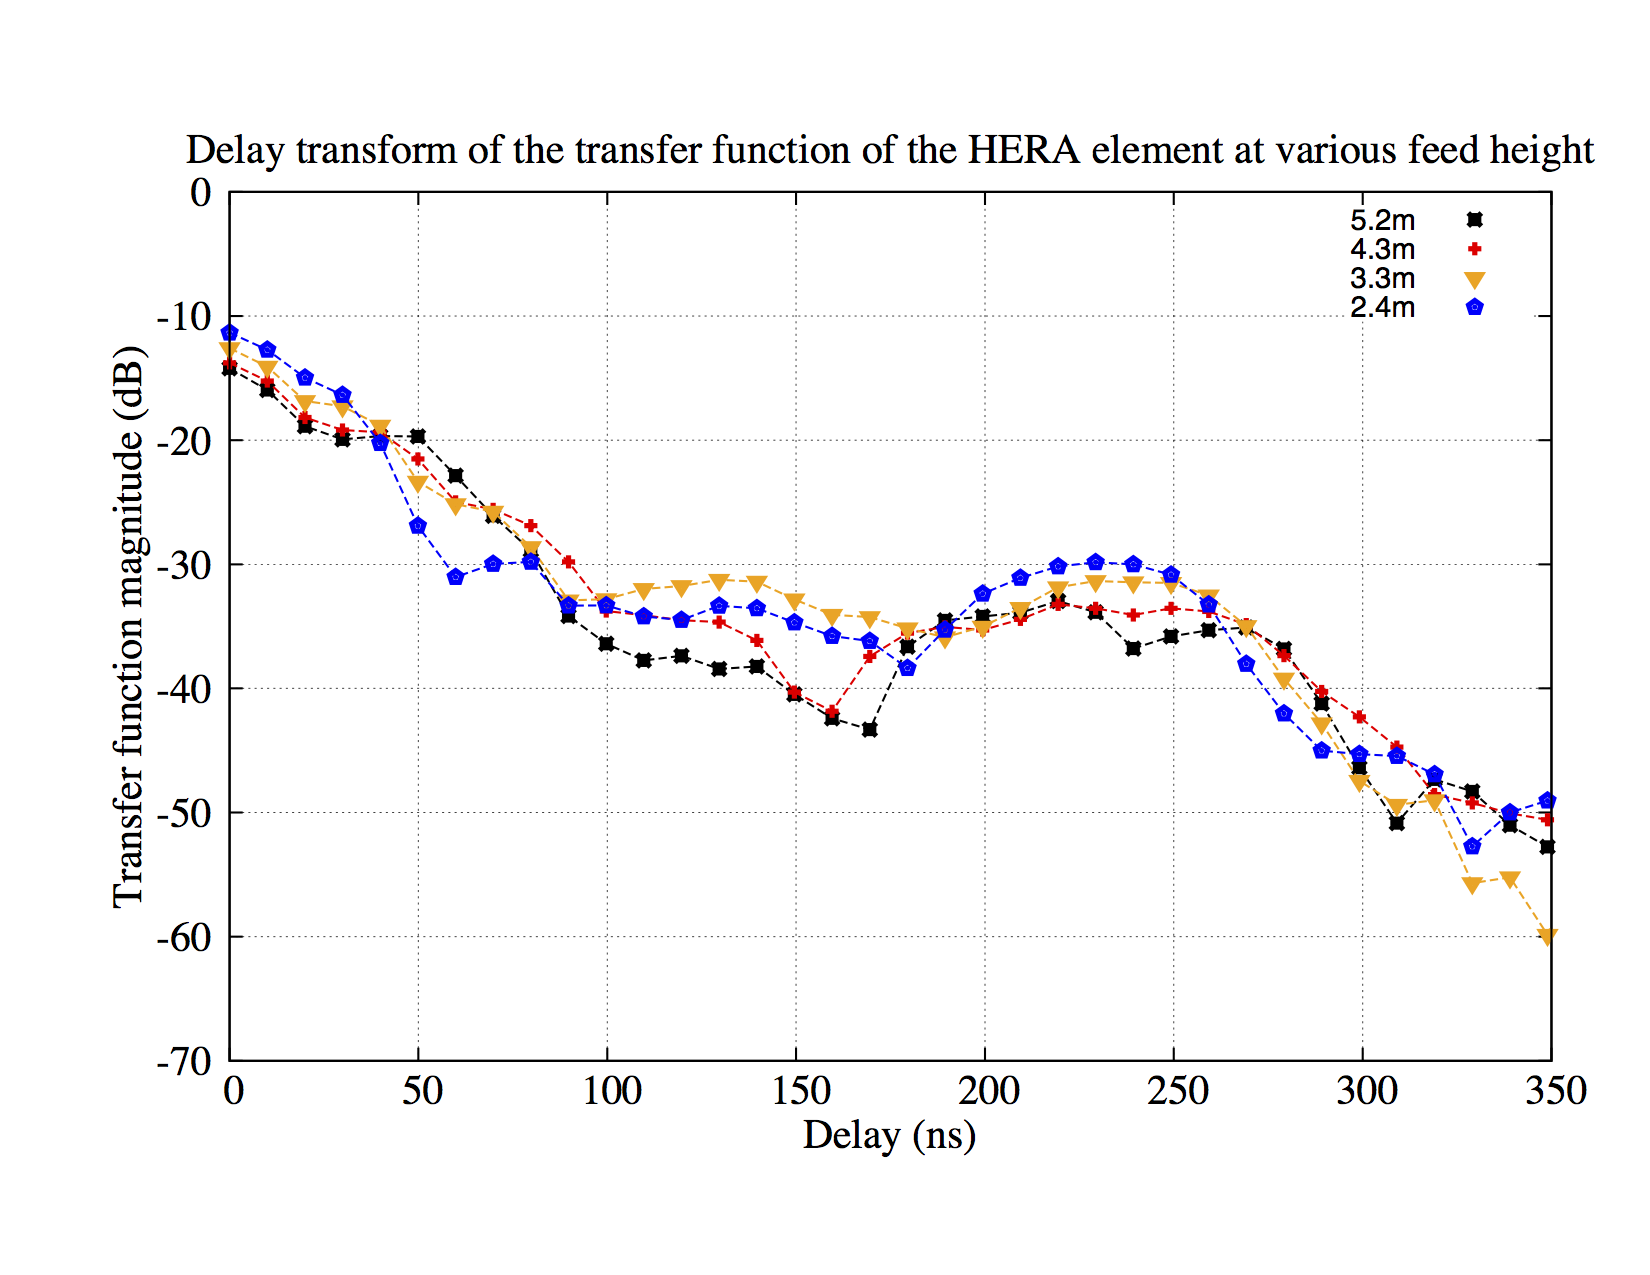
\includegraphics[width=\linewidth]{plots1/delayspectrum_height.png}
\caption{Delay transform of the transfer function of the HERA element keeping the feed at various heights. Delay transform is produced by taking the Fourier transform of the measurement using Blackman-Harris window.}
\label{fig:elevator}
\end{figure}
\begin{figure}[H]
\centering
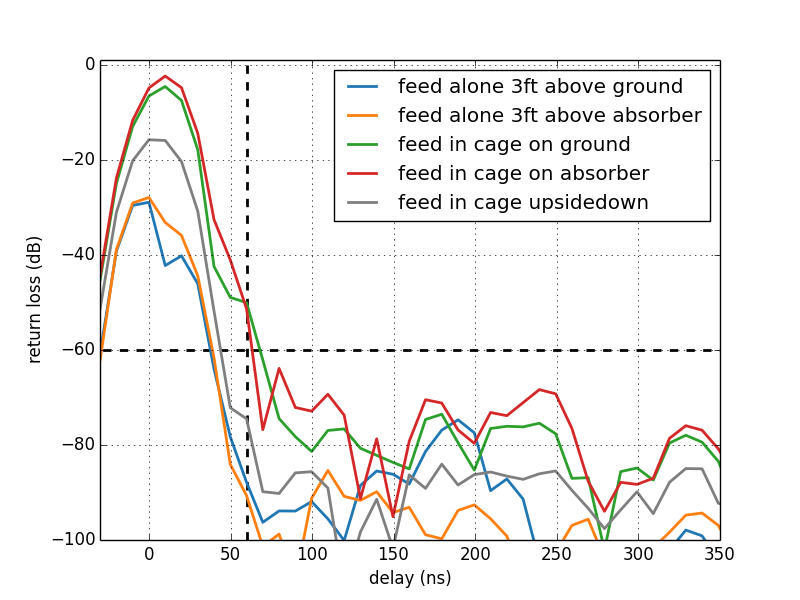
\includegraphics[width=\linewidth]{plots/delay_feed.png}
\caption{Delay plots produced using a Hamming window function for different feed only configurations and the PAPER bandwidth ($100MHz-200MHz$). The black dashed lines illustrate our ``60 by 60" specification.}
\label{fig:outofthedish}
\end{figure}

Figure \ref{fig:elevator} is again a delay plot of the return loss at four different feed suspension heights. 
We use the PAPER bandwidth and note
that the measurements are near identical at low delays, implying that low delay reflections are caused primarily by reflections within the feed cage. 
However, at higher delays we notice discrepancies between the different heights.
In addition, Figure \ref{fig:outofthedish} presents measurements taken of the feed only.away from the dish. Echosorb is placed under the feed for some of the
measurements, with the expectation that it will prevent any reflections off the
ground.
 Measurements are also taken of the feed inside its metal cage in various configurations. It is shown that the feed performs best without the cage and with the absorber. 
All these measurements are suggestive of the  fact that the feed-cage assembly itself is responsible for a significant portion of the structure up to $60ns$ and
that the cylindrical cage may be contributing up to $20ns$ to the width of the delay profile. 
We note that this depends stronglyon its coupling to structures around it. 
Structure beyond $60ns$ appears to scale with the height of the feed above the dish.



\section{Conclusion}

The delay-domain performance of the HERA dish is central to HERA's function as a power spectrum instrument.
As we have seen, reflectometry measurements can help characterize HERA's performance in this domain, and
as Equation \ref{eqn:ratio1} shows, these measurements must be adjusted for a difference in transmission/reflection
at the first feed encounter in order to be interpreted as the delay response of a feed relative to an incident
plane wave from the sky.  We also see that the choice of windowing function is critical for accurately measuring the
antenna delay response at higher delays, where sidelobes from much higher amplitude responses at small delays can easily
dominate.  We find Hamming, Hanning, and Blackman-Harris windows to be generally adequate while square windowing functions are not.
Given the critical nature of the windowing function, we recommend that all reflectometry measurements be performed in the
frequency domain, so that the data could be Fourier transformed with the appropriate window.

Taken all together, we summarize that the first version of the HERA dish, with a PAPER-style feed and cylindrical cage, is close to meeting
specification, but will require additional work to fall below $-60dB$ at $60ns$.  Given that the width of the delay response is a convolution
of the feed response and the dish reflections, it is not possible to perfectly decouple the response of the feed from that of the dish.
It may be possible to achieve enough of a reduction to meet specification by modifying the feed.
Given that previous measurements using a PAPER feed with a simple backplane exhibit structure above $-60dB$ at $60ns$,
we deduce that these advances will most likely require improving the feed return loss.  We also recommend re-investigating the scattering
cone for reducing standing waves between the feed and dish.  Finally, given the proximity of our measurements to the rough 
specification that was adopted for 
HERA of $-60dB$ attenuation at $60ns$, we recommend reinvestigating this specification to determine more accurately the impact of 
the element's current delay performance on HERA science.  We suspect that, at the level of $-50dB$ at $60ns$ and $-60dB$ at $120ns$, this
performance may indeed be adequate for the delay-domain power spectrum analysis for which HERA has been optimized.

\bibliographystyle{apj}
\bibliography{biblio.bib}
\end{document}

